\documentclass[10pt,twoside,cucitura]{toptesi}
\usepackage{lipsum}
\usepackage{hyperref}
\usepackage{tabularx}
\usepackage{framed}
\usepackage{amsmath}
\usepackage{svg}
\usepackage{graphicx}

\hypersetup{%
    pdfpagemode={UseOutlines},
    bookmarksopen,
    pdfstartview={FitH},
    colorlinks,
    linkcolor={blue},
    citecolor={red},
    urlcolor={blue}
  }

\usepackage[utf8]{inputenc}
\usepackage[T1]{fontenc}\usepackage{lmodern}

\ateneo{ITST J.F. Kennedy}
\nomeateneo{Pordenone}
\FacoltaDi{Specializzazione Informatica}
\titolo{Lupus in Tabula}
\sottotitolo{Limiti della Prima Forma Normale e NoSQL}

\candidato{\tabular{@{}l@{}}Edoardo \textsc{Morassutto}\\classe: Quinta C IA\endtabular}

\sedutadilaurea{\textsc{Anno~scolastico} 2015-2016}
\logosede{lion}

\newcommand{\role}[9]{
\begin{framed}
	\def\arraystretch{0.8}
	\begin{tabularx}{0.75\textwidth}{rX rl}
		ID			& #1 & Priorità		& #5 \\
		Nome		& #2 & Debug		& #6 \\
		Mana		& #3 & Enabled		& #7 \\
		Squadra		& #4 & Chat			& #8 \\
	\end{tabularx}
	%\vspace*{0.07cm}
	\\
	#9
\end{framed}
}

\newcommand{\gamestatus}[3]{
	\textbf{#1}: \textbf{\texttt{#2}}$\quad$ #3
}

\newcommand{\apicode}[3]{
	\texttt{#1} & \texttt{#2} & #3 \\
}

\newcommand{\eventcode}[4]{
	\textbf{#1}: \textbf{\texttt{#2}}$\quad$ #3 
	\vspace{0.1cm}
	\\
	Dati registrati dell'evento:\\
	\begin{tabular}{ll}
		#4
	\end{tabular}
	\vspace{0.2cm}
}

\begin{document}

\frontespizio

\sommario
\emph{Lupus in Tabula} è un gioco di ruolo complesso nel quale i giocatori interpretano dei personaggi e devono raccontare una storia cercando di far vincere la propria squadra. Il gioco, spesso noto anche come Mafia\cite{wiki:mafia}, si basa sul riuscire a dedurre il ruolo degli altri giocatori per capire da chi è composta la propria squadra. 

In questo documento è stato analizzato il problema di modellare i dati delle partite e di creare un server che permettesse a molti utenti di giocare in contemporanea. Durante lo sviluppo ci sono state delle difficoltà riguardo la memorizzazione di alcuni dati delle partite che sono stati in parte risolti.

Il documento è stato diviso in due parti, la prima è un'analisi completa dell'applicazione trattando nel dettaglio ogni aspetto sia progettuale che implementativo, la seconda invece, dopo un'introduzione alle forme normali, tratta delle problematiche incontrate e di alcune delle possibili soluzioni.

Durante lo sviluppo di un database \emph{relazionale} è bene cercare di rispettare le \emph{forme normali}. Una forma normale è un'insieme di regole che evitano che in una base di dati ci sia  ridondanza o inconsistenza.

In questa trattazione si esaminerà uno scenario in cui un semplice database relazionale in prima forma normale non è sufficiente a modellare il problema e si rende necessaria una diversa implementazione.

L'applicazione è stata completata ed è disponibile su \url{https://lupus.serben.tk}, tutto il sorgente è pubblico ed accessibile su \url{https://github.com/lupus-dev/lupus}.

\indici

\mainmatter

%%%%%%%%%%%%%%%%%%%%%%%%%%%%%%%%%%%%%%%%%%%%%%%%%%%%%%%
%                  PARTE UNO                          %
%%%%%%%%%%%%%%%%%%%%%%%%%%%%%%%%%%%%%%%%%%%%%%%%%%%%%%%
\part{Lupus in Tabula}


\chapter{Introduzione generale}

\section{Descrizione del gioco}
ciao mondo
Lupus in Tabula è un gioco di ruolo per, normalmente, 7 o più giocatori. Il narratore, che giocando senza computer, è un giocatore speciale che racconta una storia. La storia viene sviluppata da tutti i giocatori che, compiendo delle azioni, comportano dei cambiamenti alla vicenda, per esempio uccidendo dei personaggi o facendoli risorgere.

I giocatori sono divisi in due o più gruppi, esistono sempre le fazioni dei \emph{lupi} e dei \emph{contadini} alle quali può aggiungersi quella dei \emph{criceti mannari} ed altre. Quando la partita finisce solo una di queste squadre vince.

Lo scopo della squadra dei \emph{lupi} è quello di sbranare tutti gli altri giocatori, mentre quello dei \emph{contadini} è di individuare ed uccidere tutti i \emph{lupi}.

La partita si alterna di giorni e di notti, durante ogni notte tutta la squadra dei lupi deve scegliere un bersaglio (solitamente un contadino) che quella notte verrà sbranato. Durante il giorno, invece, ogni giocatore deve votare chi, secondo lui, mandare al rogo. Questo è l'unico modo per i contadini di uccidere i vari lupi che si aggirano nel villaggio. A questa votazione partecipano anche i lupi che cercheranno ovviamente di non farsi votare.

Per rendere il gioco più dinamico vengono inseriti tra i giocatori alcuni ruoli speciali. Per esempio un \emph{veggente} è un contadino che, durante la notte, può scegliere un giocatore vivo e, tramite consultazione della palla di cristallo, sapere se ha un'anima buona oppure cattiva. Ogni ruolo infatti, oltre ad essere di una certa squadra, ha anche delle caratteristiche extra come il \emph{mana}, che può essere buono oppure cattivo. Normalmente (ma non necessariamente) i giocatori nella squadra dei lupi hanno mana cattivo mentre quelli nella squadra dei contadini ce l'hanno buono.

Ogni giocatore, in generale, conosce solo il proprio ruolo e deve dedurre quello degli altri giocatori; ci possono essere dei casi in cui qualche giocatore conosce il ruolo esatto di qualcun altro. Per esempio ogni lupo conosce esattamente quali sono i suoi compagni di squadra.

Quanto un giocatore muore in una partita normale è il narratore ad annunciarlo, in questa implementazione è presente un giornale nel quale viene scritto il nome dei giocatori che sono morti.

Affinchè una partita termini correttamente deve verificarsi alemno una delle seguenti condizioni:

\begin{itemize}
	\item Tutti i giocatori sono morti
	\item Almeno una fazione ha vinto
	\begin{itemize}
		\item Lupi: Il numero di lupi è maggiore o uguale al numero di contadini
		\item Contadini: Il numero di lupi è zero
	\end{itemize}
\end{itemize}

\section{Ruoli}
Ad ogni giocatore viene assegnato dal sistema uno ed un solo ruolo, quindi il giocatore saprà anche la sua fazione e il suo mana. 

Ogni ruolo, oltre al nome ha anche alcune proprietà aggiuntive:

\begin{itemize}
	\item Mana: indica se il giocatore agirà come malintenzionato oppure come una brava persona
	\item Nome identificativo: nome unico che identifica il ruolo
	\item Priorità: serve per stabilire un ordine nell'esecuzione delle azioni
	\item Debug: alcuni ruoli sono accessibili solo dagli sviluppatori e sono marcati come \emph{debug}
	\item Enabled: È possibile disattivare alcuni ruoli con questa proprietà
	\item Chat: alcuni ruoli hanno dei canali di comunicazione dedicati
	\item Gen*: parametri aggiuntivi per la generazione automatica dei ruoli, come numero minimo e massimo di occorrenze del ruolo, probabilità, ecc...
\end{itemize}

\subsection{Ruoli comuni}

I ruoli che normalmente vengono usati in una partita di Lupus in Tabula sono:

\role{Lupo}{Lupo}{Cattivo}{Lupi}{100}{no}{sì}{Lupi}{Durante la notte i \emph{lupi} votano chi eliminare, se almeno il 50\%+1 dei \emph{lupi} vivi votano la stessa persona, questa è una candidata a morire}

\role{Guardia}{Guardia}{Buono}{Contadini}{10000}{no}{si}{}{Durante la notte la \emph{guardia} può scegliere di proteggere una persona, se i \emph{lupi} quella notte decidessero di ucciderla, essa non muore}

\role{Medium}{Medium}{Buono}{Contadini}{150}{no}{si}{}{Il \emph{medium} durante la notte può scegliere di guardare un giocatore morto, lui saprà se quel giocatore aveva un mana buono o cattivo}

\role{Paparazzo}{Paparazzo}{Buono}{Contadini}{1000}{no}{si}{}{Il \emph{paparazzo} durante la notte sceglie una persona da pedinare, vengono riportati sul giornale della mattina seguente tutti i giocatori che hanno visitato il personaggio \textsl{paparazzato}}

\role{Criceto mannaro}{Criceto mannaro}{Cattivo}{Criceti}{10000}{no}{si}{}{\'E un giocatore normale, senza poteri speciali. Se la partita termina e lui è ancora vivo allora vince solo lui e non la sua fazione}

\role{Assassino}{Assassino}{Cattivo}{Contadini}{10}{no}{si}{}{L'\emph{assassino} una sola volta nella partita può scegliere una persona e ucciderla}

\role{Massone}{Massone}{Buono}{Contadini}{10000}{no}{si}{Massoni}{I \emph{massoni} non hanno poteri però hanno una chat dedicata e quindi si conoscono tra loro}

\role{Contadino}{Contadino}{Buono}{Contadini}{10000}{no}{si}{}{I \emph{contadini} non hanno poteri\dots}

\role{Pastore}{Pastore}{Buono}{Contadini}{50}{sì}{si}{}{I \emph{pastori} possono scegliere di sacrificare delle pecore per salvare dei giocatori dalle grinfie dei lupi}

\role{Sindaco}{Sindaco}{Buono}{Contadini}{10000}{no}{si}{}{Il \emph{sindaco} è un contadino che non può essere messo al rogo nella votazione diurn}

\chapter{Analisi}

\section{Analisi del problema}
È necessario sviluppare un sistema robusto che gestisce gli utenti e le partite di Lupus in Tabula.

Il sistema deve essere in grado di sopportare un numero crescente di giocatori e un numero molto elevato di partite, deve essere in grado di scalare ottimalmente con le richieste. La base di dati deve essere sviluppata in modo da garantire un funzionamento efficiente e una robustezza dei dati.

I dati identificativi degli utenti devono essere conservati in modo sicuro, è necessario proteggere le credenziali di accesso tramite avanzati sistemi di \emph{hashing}.

È necessario fare molta attenzione ai privilegi degli utenti, proteggendo le risorse che non sono accessibili. Per esempio è opportuno evitare che gli utenti possano vedere, entrare o modificare le partite alle quali gli è stato negato il permesso.

Le chiavi interne del database non sono visibili agli utenti, delle chiavi alternative non numeriche sono visualizzate dagli utenti. Per esempio le partite non vengono identificate (lato utente) da un intero progressivo ma da un \emph{nome breve}, una sequenza di caratteri che rispetta la seguente \texttt{regex}: \texttt{[a-zA-Z][a-zA-Z0-9]\{0,9\}}. Deve essere lungo da 1 a 10 caratteri \texttt{ASCII}, il primo carattere deve essere una lettera e deve essere unico nel suo contesto.

\section{Stuttura dei componenti}
Ogni utente registrato nel sistema può giocare alle partite create dagli altri giocatori oppure può creare delle sue partite. Per creare delle partite l'utente deve creare delle staze, dei raggruppamenti di zero, una o più partite.

Una stanza appartiene ad uno ed un solo utente che ha poteri amministrativi su questa, solo lui può creare una nuova partita in quella stanza. Ogni stanza viene identificata da un \emph{nome breve} univoco e non modificabile ed ha una breve descrizione. In una stanza ci può essere al più una parita in corso.

Quando un utente possiede una stanza libera (senza partite in corso), può decidere di creare una nuova partita, questa viene identificata da un \emph{nome breve} univoco all'interno della stanza ma non globalmente e non modificabile. La partita ha anche una breve descrizione.

Gli altri utenti possono entrare nella partita solo se hanno i permessi per farlo, ogni partita infatti condivide i permessi della stanza a cui appartiene, per esempio se la stanza è protetta da delle liste di accesso (\texttt{ACL}), solo gli utenti specificati possono accedervi.

Una partita è composta da una serie di giocatori, degli utenti a cui è stato assegnato un ruolo (eventualmente non definito). Appena un giocatore entra nella partita (e questa non è iniziata) gli viene assegnato un ruolo non definito (\texttt{unknown}). Appena il numero di giocatori raggiunge il valore specificato dall'amministratore vengono generati i ruoli esatti dei giocatori. I ruoli possono essere generati in due modi: manualmente secondo precise impostazioni dell'amministratore oppure automaticamente specificando solo quali ruoli generare.

Ogni utente può giocare anche a diverse partite in contemporanea, in accordo con i limiti imposti dal suo livello. Ogni utente infatti ha un livello che limita le sue possibilità di gioco, come il numero di partite contemporanee, il numero di stanze e il numero di stanze private.

Il livello di un giocatore è sempre crescente, si può venire declassati solo dall'amministratore del server. Il livello viene stabilito tramite un valore detto \emph{karma} che rappresenta un'indicazione del tempo di gioco dell'utente. Si guadagnano punti karma giocando partite, vincendo partite o invitando altri giocatori. Quando il karma raggiunge un valore sufficientemente alto viene aumentato il livello dell'utente. 

Per porter usare le funzionalità in beta è necessario possedere un livello sufficientemente alto.

Il livello di un utente è visibile nella pagina dell'utente e in ogni partita viene evidenziato. I possibili livelli sono:

\begin{tabular}{|c|c|c|c|c|c|c|}
	\hline
	& \textbf{Nome} & \textbf{Karma} & \textbf{Partite parallele} & \textbf{Stanze} & \textbf{Stanze private} & \textbf{BETA} \\
	\hline
	1 & Neofita 	 & 0    &   3 &   1 &   0 & no \\
	2 & Principiante & 25   &   5 &   1 &   0 & no \\
	3 & Gamer        & 50   &   5 &   3 &   1 & no \\
	4 & Esperto      & 100  &   5 &   5 &   3 & no \\
	5 & Maestro      & 200  &   7 &   5 &   5 & no \\
	6 & ProGamer     & 500  &  10 &  10 &   5 & no \\
	7 & Stratega     & 2000 &  15 &  10 &  10 & si \\
	8 & Generale     & 5000 &  50 & 100 &  10 & si \\
	9 & Guru         & 10000& 100 & 100 & 100 & si \\
	10 & GameMaster   & $\infty$ & 1000 & 1000 & 1000 & si \\
	\hline
\end{tabular}

\section{Progettazione della base di dati}
Come analizzato nella Seconda Parte [\ref{sec:soluzione}] il database è stato diviso in due parti, una relazionale e una \texttt{NoSQL}. In relazione alla parte relazionale è qui proposto uno schema Entità-Relazione.

Alcuni attributi sono stati mantenuti dal passaggio dalla prima versione del Database (senza NoSQL) a quella più recente. In particolare tutti gli attributi che non rispettavano la Prima Forma Normale sono stati lasciati ed ora sono facoltativi (se lasciati a \texttt{NULL} viene usata la versione in NoSQL).

Tutto ciò sia per retrocompatibilità che per garantire il funzionamento della piattaforma anche in eventuali servizi di hosting che non supportano NoSQL.

\subsection{Schema concettuale}
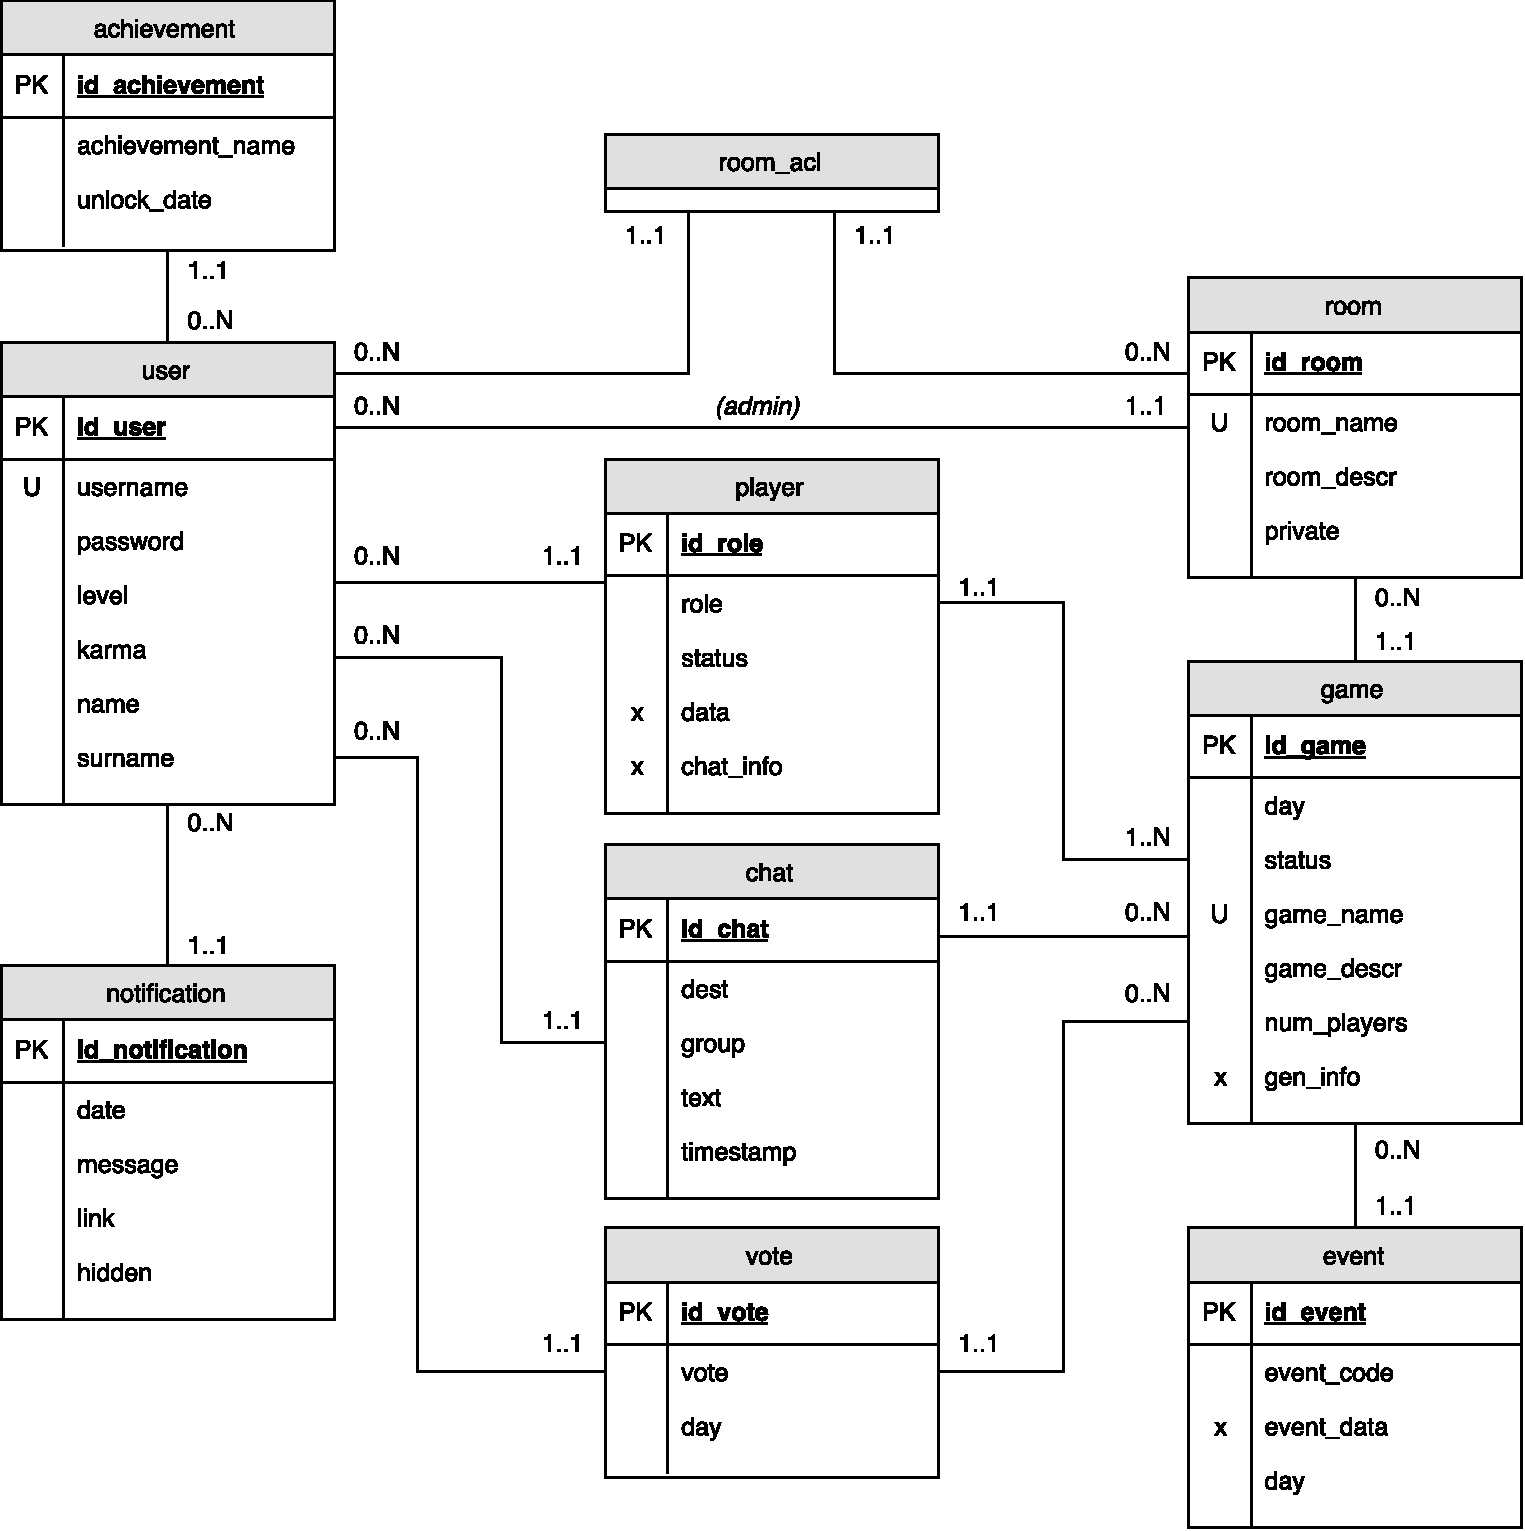
\includegraphics[width=\textwidth]{ER.pdf}

\subsection{Schema logico}
Vengono qui riportate, in modo sintetico le definizioni di tutte le tabelle che compongono la base di dati. Le chiavi primarie sono \underline{sottolineate}, le chiavi esterne sono in \emph{corsivo} con il relativo riferimento; i campi ristrutturati con NoSQL hanno un asterisco ($^*$).

\begin{itemize}
	\item \texttt{user(\underline{id\_user}, username, password, level, karma, name, surname)}
	\item \texttt{room(\underline{id\_room}, \emph{id\_admin}\extkey{user.id\_user}, room\_name, room\_descr, private)}
	\item \texttt{game(\underline{id\_game}, \emph{id\_room}\extkey{room.id\_room}, day, status, game\_name, game\_descr, \\num\_players, gen\_info$^*$)}
	\item \texttt{player(\underline{id\_role}, \emph{id\_game}\extkey{game.id\_game}, \emph{id\_user}\extkey{user.id\_user}, role, status, data$^*$, \\chat\_info$^*$)}
	\item \texttt{chat(\underline{id\_chat}, \emph{id\_game}\extkey{game.id\_game}, \emph{id\_user\_from}\extkey{user.id\_user}, dest, group, text, \\timestamp)}
	\item \texttt{vote(\underline{id\_vote}, \emph{id\_game}\extkey{game.id\_game}, \emph{id\_user}\extkey{user.id\_user}, vote, day)}
	\item \texttt{event(\underline{id\_event}, \emph{id\_game}\extkey{game.id\_game},  event\_code, event\_data$^*$, day)}
	\item \texttt{notification(\underline{id\_notification}, \emph{id\_user}\extkey{user.id\_user}, date, message, link, hidden)}
	\item \texttt{achievement(\underline{id\_achievement}, \emph{id\_user}\extkey{user.id\_user}, achievement\_name, unlock\_date)}
	\item \texttt{room\_acl(\underline{\emph{id\_room}}\extkey{room.id\_room}, \underline{\emph{id\_user}}\extkey{user.id\_user})}
\end{itemize}

\subsection{Descrizione delle entità}
$\rightarrow$ inserire descrizione entità $\leftarrow$

\subsection{Dizionario degli attributi}
$\rightarrow$ inserire dizionario degli attributi $\leftarrow$

\section{Codici utilizzati}
Nel gioco, per alleggerire la base di dati e per snellire il tutto sono state usate delle convenzioni riguardo alcuni codici. Per esempio per evitare di memorizzare un'intera stringa come \texttt{Giorno 4} è stato scielto di memorizzare l'intero 6, mentre per la \texttt{Notte 1} il valore 1.

Questi codici sono qui riportati e descritti e sono modificabili sono andando ad intervenire nella apposite classi dedicate alla sola memorizzazione di queste costanti. Questi valori non sono stati usati semplicemente nel codice ma viene sempre fatto riferimento alle costanti specificate.

\subsection{Tempo del gioco}
Come appena preannunciato il tempo di una partita viene semplicemente memorizzato come numero intero secondo la seguente convenzione:

\[
day
\left\{
\begin{aligned}
\text{se}\ day = 0 						&\Rightarrow \text{arrivo al villaggio} \\
\text{se}\ day\ \text{è \emph{pari}}		&\Rightarrow \text{giorno}\ \frac{day}{2}+1 \\
\text{se}\ day\ \text{è \emph{dispari}}	&\Rightarrow \text{notte}\ \frac{day}{2}+1
\end{aligned}
\right.
\]

Il valore di \emph{day} viene memorizzato nella tabella game in quanto si tratta del giorno della partita.

Sono qui riportati degli esempi dei valori che può assumere \emph{day}:

\begin{tabular}{|c|c|}
	\hline
	\textbf{day} & \textbf{valore} \\
	\hline
	0 & Arrivo al villaggio \\
	1 & Notte 1 \\
	2 & Giorno 2 \\
	3 & Notte 2 \\
	4 & Giorno 3 \\
	5 & Notte 3 \\
	6 & Giorno 4 \\
	7 & Notte 4 \\
	\hline
\end{tabular}

\subsection{Stato della partita}
Ogni partita deve trovarsi in uno stato preciso che indica le condizioni della partita. In particolare è necessario sapere se la partita è già iniziata, se è finita, se ha vinto una certa squadra, se è stata interrotta ecc...

Per rendere più chiaro il valore di questi codici i vari stati delle partite sono stati divisi in alcune fasi: Pre-Partita, In-Partita, Terminata-OK, Terminata-Errore.

\subsubsection{Fase Pre-Partita}
Questa fase è presente solo prima dell'avvio della partita e serve per salvare ed aggiustare i dettagli della partita, come il numero di giocatori, di ruoli, la descrizione, ecc\dots

Questa fase è identificata da codici nell'intervallo:
\[
0 \le x < 100
\]

I codici riconosciuti sono:
\begin{itemize}
	\item \gamestatus{0}{Setup}{Impostazione della partita}
\end{itemize}


\subsubsection{Fase In-Partita}
Questa fase è presente poco prima dell'inizio della partita e durante tutto il corso della partita. 

Viene identificata da codici nell'intervallo:
\[
100 \le x < 200
\]

I codici riconosciuti sono:
\begin{itemize}
	\item \gamestatus{100}{NotStarted}{La partita è attiva e i giocatori possono iniziare ad entrare}
	\item \gamestatus{101}{Running}{La partita è in corso e i giocatori non possono più entrare}
\end{itemize}


\subsubsection{Fase terminata in modo corretto}
Questa fase si verifica quando la partita termina in modo corretto e viene scelta una squadra vincitrice.

I codici che la identificano sono compresi nell'intervallo:
\[
200 \le x < 300
\]

I codici riconosciuti sono:
\begin{itemize}
	\item \gamestatus{200\,+\,y}{Win$y$}{La partita è terminata e ha vinto la squadra $y\ (0\le y < 99)$}
	\item \gamestatus{299}{DeadWin}{La partita è terminata perché tutti i giocatori sono morti}
\end{itemize}



\subsubsection{Fase terminata in modo inaspettato}
Questa fase si verifica quando la partita viene interrotta prima della sua normale fine. In questo caso non viene designato alcun vincitore.

I codici che identificano questa fase sono compresi dall'intervallo:
\[
300 \le x < 400
\]

I codici riconosciuti sono:
\begin{itemize}
	\item \gamestatus{300}{TermByAdmin}{L'amministratore della stanza ha fatto terminare la partita}
	\item \gamestatus{301}{TermBySolitude}{Un numero eccessivo di giocatori hanno abbandonato la partita}
	\item \gamestatus{302}{TermByVote}{\'E stato raggiunto il \emph{quorum} per terminare la partita}
	\item \gamestatus{303}{TermByBug}{Un errore interno del server ha fatto terminare la partita per preservare l'integrità del server}
	\item \gamestatus{304}{TermByGameMaster}{Il GameMaster ha deciso di terminare la partita}
\end{itemize}

\subsection{Codici di risposta delle API}
Le funzioni delle API ritorneranno un codice numerico identificativo del messaggio di errore/successo che la relativa funzione ha avuto. 

I codici sono divisi in gruppi di decine: le unità sono un numero progressivo che identifica la sezione caratterizzata dalle altre cifre del codice.

\resizebox{\textwidth}{!} {
\begin{tabular}{|rl|l|}
\hline
\textbf{\#} & \textbf{Abbreviazione} & \textbf{Descrizione} \\
\hline
\apicode{1}{NotLoggedIn}{L'utente non è connesso e non può accedere a questa risorsa}
\apicode{2}{FatalError}{Un errore grave interno al server può aver compromesso la partita}
\apicode{3}{AccessDenied}{L'utente non ha i permessi per accedere alla risorsa richiesta}
\apicode{4}{NotFound}{La risorsa richiesta non è stata trovata}
\apicode{5}{MissingParameter}{Non è stato specificato un parametro richiesto}
\apicode{6}{MalformedParameter}{Uno dei parametri non ha un formato corretto o è invalido}
\apicode{7}{Done}{La richiesta è stata completata con successo}
\apicode{8}{Fail}{La richiesta non è stata completata a causa di un errore}
\apicode{9}{Found}{La risorsa è stata trovata}
\hline
\apicode{101}{LoginAlreadyDone}{Utente già connesso}
\hline
\apicode{130}{JoinDoneGameStarted}{L'utente è entrato nella partita e questa è iniziata}
\apicode{131}{JoinDoneGameWaiting}{L'utente è entrato nella partita ma questa è in attesa}
\apicode{132}{JoinFailedAlreadyIn}{L'utente era già entrato nella partita}
\apicode{133}{JoinFailedGameClose}{Non sono permessi ingressi}
\apicode{134}{JoinFailedGameFull}{L'utente non è entrato nella partita perché è piena}
\apicode{135}{JoinFailedGamesEnded}{La partità era finita, il giocatore non è entrato}
\hline
\apicode{143}{NewGameAlreadyRunning}{Una partita nella stanza è ancora in corso}
\apicode{144}{NewGameAlreadyExists}{Esiste già una partita con questo nome nella stanza}
\hline
\apicode{152}{StartNotInSetup}{La partita non è in fase di setup}
\apicode{153}{StartWithoutLupus}{La partita non contiene lupi}
\hline
\apicode{160}{VoteDoneNextDay}{La votazione è stata effettuata e la partita è avanzata}
\apicode{161}{VoteDoneWaiting}{La votazione è stata effettuata e la partita è in attesa}
\apicode{162}{VoteDoneGameEnd}{La votazione è stata effettuata e la partita è terminata}
\apicode{164}{VoteGameNotRunning}{La partita non è in corso}
\apicode{166}{VoteNotValid}{Il voto dell'utente non è valido}
\apicode{167}{VoteNotNeeded}{L'utente non deve votare o ha già votato}
\hline
\apicode{172}{NewRoomRoomsEnded}{L'utente ha finito il numero di stanze che può creare}
\apicode{173}{NewRoomPrivateRoomsEnded}{L'utente ha finito il numero di stanze private che può creare}
\apicode{174}{NewRoomAlreadyExists}{Esiste già una stanza con questo nome}
\hline
\apicode{200}{CheckRoomNameAccepted}{Il nome della stanza è corretto ed accettabile}
\apicode{203}{CheckRoomNameExisting}{Il nome della stanza è già stato usato}
\hline
\apicode{210}{CheckRoomDescrAccepted}{La descrizione della stanza è accettabile}
\hline
\apicode{220}{CheckGameNameAccepted}{Il nome della partita è corretto ed accettabile}
\apicode{224}{CheckRoomNameExisting}{Il nome della partita è già stato usato in questa stanza}
\hline
\apicode{230}{CheckGameDescrAccepted}{La descrizione della partita è accettabile}
\hline
\apicode{242}{SetupNotInSetup}{La partita non è in fase di setup}
\hline
\apicode{252}{SignupAlreadyExists}{Non è possibile registrare un utente con questo \texttt{username}}
\hline
\apicode{263}{ChatUserNotInGame}{L'utente non è nella partita}
\apicode{264}{ChatInvalidUser}{Il destinatario del messaggio non è valido}
\hline
\apicode{270}{GameTerminated}{La partita è stata terminata dall'amministratore}
\apicode{272}{GameTermNotRunning}{La partita non era in corso}
\hline
\apicode{282}{PlayerKickNotValidState}{La partita non è in uno stato valido per espellere giocatori}
\hline
\apicode{290}{ACLAlreadyPresent}{La regola ACL era già presente nell'elenco}
\apicode{291}{ACLCannotRemoveAdmin}{Non è possibile rimuovere l'admin della stanza dall'ACL}
\hline
\end{tabular}
}

Non tutte le decine sono state usate in quanto, durante lo sviluppo, alcuni codici sono stati rimossi.

\subsection{Codici degli eventi}
Gli eventi che si verificano nella partita vengono memorizzati per essere visualizzati nel giornale del villaggio. Questi eventi vengono distinti in base ad un codice numerico che identifica il tipo di evento. Ad ogni tipologia di evento corrispondono alcuni attributi specifici, come per esempio lo username del giocatore ucciso o dell'assassino o una lista degli username dei giocatori visti.

\begin{itemize}
\item \eventcode{0}{GameStart}{La partita è appena iniziata}{
\texttt{players} & Vettore con gli \texttt{username} dei giocatori nella partita \\
\texttt{start}   & Timestamp dell'ora dell'inizio della partita
}
\item \eventcode{1}{Death}{Un giocatore è stato ucciso o è stato trovato morto}{
\texttt{dead}	& Username del giocatore morto \\
\texttt{cause}	& Causa della morte \\
\texttt{actor}	& Causante della morte (killer)
}
\item \eventcode{2}{MediumAction}{Un medium ha guardato un morto}{
\texttt{medium}	& Username del medium \\
\texttt{seen}	& Username del giocatore guardato \\
\texttt{mana}	& Mana del giocatore guardato
}
\item \eventcode{3}{VeggenteAction}{Un veggente ha guardato un vivo}{
\texttt{medium}	& Username del veggente \\
\texttt{seen}	& Username del giocatore guardato \\
\texttt{mana}	& Mana del giocatore guardato
}
\item \eventcode{4}{PaparazzoAction}{Un paparazzo ha fotografato un giocatore}{
\texttt{paparazzo}	& Username del paparazzo \\
\texttt{seen}	    & Username del giocatore guardato \\
\texttt{visitors}   & Lista dei giocatori che hanno fatto visita al giocatore
}
\item \eventcode{5}{BecchinoAction}{Un becchino ha resuscitato un giocatore}{
\texttt{becchino}	& Username del becchino \\
\texttt{dead}	    & Username del giocatore resuscitato
}
\item \eventcode{6}{PlayerKicked}{Un giocatore è stato espulso dalla partita}{
\texttt{kicked}	& Username del giocatore espulso
}
\end{itemize}

\subsection{Visibilità della stanza}
Una stanza può essere resa privata dall'amministratore. Esistono 3 livelli di visibilità di una stanza:

\begin{enumerate}
	\setcounter{enumi}{-1}
	\item \textbf{Pubblica}: la stanza è accessibile a chiunque ed è elencata nell'elenco delle partite
	\item \textbf{Solo link}: la stanza è accessibile a chiunque possegga il link, non viene elencata
	\item \textbf{Privata}: solo gli utenti specificati dall'amministratore della stanza possono vederla e solo loro la vedono negli elenchi
\end{enumerate}

\chapter{Implementazione}

\section{Tecnologie utilizzate}
\section{Pagine web}
\section{Webservice REST}

%%%%%%%%%%%%%%%%%%%%%%%%%%%%%%%%%%%%%%%%%%%%%%%%%%%%%%%
%                  PARTE DUE                          %
%%%%%%%%%%%%%%%%%%%%%%%%%%%%%%%%%%%%%%%%%%%%%%%%%%%%%%%
\part{Limiti della 1NF}

\chapter{Introduzione alle forme normali}

\section{Prima forma normale}
\section{Seconda forma normale}
\section{Terza forma normale}
\section{Forma normale di Boyce-Codd}
\section{Quarta e Quinta forma normale}

\chapter{Problematiche con la 1NF}

\section{Contesto del problema}

\section{Prime soluzioni parziali}
\subsection{Una tabella per ruolo}
\subsection{Una tabella key-value}

\section{Soluzione proposta}
\label{sec:soluzione}

\end{document}
